\documentclass[a4paper,12pt]{article}

\usepackage[utf8]{inputenc}
\usepackage[english]{babel}
\usepackage{graphicx}
\usepackage{amsmath}
\usepackage{amsfonts}
\usepackage{amssymb}
\usepackage{geometry}
\usepackage{hyperref}
\usepackage{listings}
\usepackage{color}
\usepackage{booktabs}
\usepackage{float}
\usepackage{caption}

% Configurazione margini
\geometry{top=3cm, bottom=3cm, left=2.5cm, right=2.5cm}

% Configurazione per il codice
\definecolor{codegreen}{rgb}{0,0.6,0}
\definecolor{codegray}{rgb}{0.5,0.5,0.5}
\definecolor{codepurple}{rgb}{0.58,0,0.82}
\definecolor{backcolour}{rgb}{0.95,0.95,0.92}

\lstdefinestyle{mystyle}{
    backgroundcolor=\color{backcolour},   
    commentstyle=\color{codegreen},
    keywordstyle=\color{magenta},
    numberstyle=\tiny\color{codegray},
    stringstyle=\color{codepurple},
    basicstyle=\ttfamily\footnotesize,
    breakatwhitespace=false,         
    breaklines=true,                 
    captionpos=b,                    
    keepspaces=true,                 
    numbers=left,                    
    numbersep=5pt,                  
    showspaces=false,                
    showstringspaces=false,
    showtabs=false,                  
    tabsize=2
}

\lstset{style=mystyle}

\begin{document}

% --- FRONTESPIZIO ---
\begin{titlepage}
    \centering
    \vspace*{1cm}
    
    {\LARGE \textbf{Università degli Studi di Siena} \par}
    \vspace{1.5cm}
    
    {\Large \textbf{Project title: Performance Analysis of SpMV using CUDA, OpenMP and Advanced Formats (JDS, Hybrid)} \par}
    \vspace{1.5cm}
    {\large \textbf{Student:}}
    {\large Giovanni Paolo Maugeri (matr. 165194) \par}
    {\large  Valentino Basili (matr. #aggiungi matricola#) \par}
    \vspace{1cm}
    
    {\large \textbf{Professor:} Roberto Giorgi \par}
    
    \vfill
    
    {\large Academic Year 2025/2026 \par}
\end{titlepage}

% --- INDICE ---
\tableofcontents
\newpage

% --- CONTENUTO ---

\section{Introduction}
\subsection{Overview}
The objective of this project is to analyze and compare the performance of the Sparse Matrix-Vector Multiplication (SpMV) kernel across different architectures and storage formats. SpMV is a fundamental building block in many scientific computing applications, defined as $y = Ax$, where $A$ is a sparse matrix and $x, y$ are dense vectors.

Since the operation is strictly memory-bound, the choice of the storage format significantly impacts the effective bandwidth utilization. We implemented and tested the algorithm using \textbf{CUDA} (for GPU acceleration), \textbf{OpenMP} (for CPU parallelism), and a sequential C++ baseline. 

We analyzed four main storage formats, specifically chosen to handle different sparsity patterns:
\begin{enumerate}
    \item \textbf{CSR} (Compressed Sparse Row) - The standard baseline.
    \item \textbf{ELL} (ELLPACK) - Optimized for structured grids on GPU.
    \item \textbf{Hybrid} (ELL + COO) - A combination to handle moderate irregularity.
    \item \textbf{JDS} (Jagged Diagonal Storage) - A technique to minimize warp divergence on GPUs.
\end{enumerate}

\section{Sparse Matrix Formats}

\subsection{CSR (Compressed Sparse Row)}
The CSR format utilizes three arrays to compress the row indices, making it the standard format for sparse linear algebra on CPUs.

\begin{itemize}
    \item \textbf{Arrays \& Structure:}
    \begin{itemize}
        \item \texttt{Value}: An array of size $NNZ$ (number of non-zeros) storing the non-zero elements contiguously.
        \item \texttt{Column}: An array of size $NNZ$ mapping each element in \texttt{Value} to its column index.
        \item \texttt{RowPtrs}: An array of size $N + 1$ (where $N$ is the number of rows). It stores the starting index in \texttt{Value} for each row. The last element points to the end of the array (equal to $NNZ$).
    \end{itemize}
    
    \item \textbf{Pros:} Efficient memory usage ($2 \cdot NNZ + N + 1$ storage); very fast for Matrix-Vector Multiplication (SpMV) on CPUs.
    \item \textbf{Cons:} Difficult to modify (inserting elements requires shifting arrays); on GPUs, it can cause load imbalance if row lengths vary significantly (some threads work much longer than others).
\end{itemize}



\subsection{ELL (ELLPACK)}
ELL fits the sparse matrix into a dense $N \times K$ structure, where $K$ is the maximum number of non-zeros in any single row. Rows with fewer than $K$ elements are padded with a sentinel value (usually zero).

\begin{itemize}
    \item \textbf{Arrays \& Structure:}
    \begin{itemize}
        \item \texttt{Value}: A dense 2D array of dimensions $N \times K$ (often stored in Column-Major order on GPUs).
        \item \texttt{Index}: A dense 2D array of dimensions $N \times K$ storing the column indices. Padded entries usually store a dummy index.
    \end{itemize}

    \item \textbf{Pros:} Perfect memory coalescing on GPUs (if Column-Major); removes the need for row pointers, allowing uniform control flow.
    \item \textbf{Cons:} Extremely inefficient for irregular matrices. If one row is very long ($max\_nnz \gg avg\_nnz$), the format allocates massive amounts of memory for padding zeros.
\end{itemize}



\subsection{Hybrid (ELL + COO)}
To mitigate the memory waste of ELL, the Hybrid format splits the matrix into two parts: a regular ELL portion and an overflow COO portion.

\begin{itemize}
    \item \textbf{Arrays \& Structure:}
    \begin{itemize}
        \item \textbf{ELL Part:} Uses standard ELL arrays (\texttt{Value}, \texttt{Index}) of size $N \times K_{cutoff}$, where $K_{cutoff}$ covers the majority of rows.
        \item \textbf{COO Part:} Uses three arrays (\texttt{Row}, \texttt{Col}, \texttt{Val}) to store the "overflow" elements for rows longer than $K_{cutoff}$.
    \end{itemize}

    \item \textbf{Pros:} Balances the high bandwidth of ELL with the flexibility of COO; effectively handles "power-law" matrices (many short rows, few very long rows).
    \item \textbf{Cons:} Higher implementation complexity (requires separate kernels or logic for each part); performance overhead when merging results from the two partitions.
\end{itemize}



\subsection{JDS (Jagged Diagonal Storage)}
JDS is explicitly designed to solve the Warp Divergence problem on GPUs by reordering the matrix rows.

\begin{itemize}
    \item \textbf{Arrays \& Structure:}
    \begin{itemize}
        \item \texttt{Permutation}: An array of size $N$ storing the mapping of original row indices to the sorted row indices.
        \item \texttt{JD\_Ptr}: An array pointing to the start of each "jagged diagonal" (iteration).
        \item \texttt{Value} \& \texttt{Col}: Arrays storing the non-zeros and column indices, ordered first by the jagged diagonal, then by the sorted row.
    \end{itemize}

    \item \textbf{Pros:} Minimizes warp divergence on GPUs (threads in a warp process rows of similar length); ensures balanced workload.
    \item \textbf{Cons:} High preprocessing cost (sorting rows); requires gathering results back to original row positions (indirect memory access via the permutation array).
\end{itemize}

\newpage
\section{Implementation Details}

\subsection{Data Layout: Row-Major vs Column-Major}
A critical optimization identified during development is the memory layout dependency on the architecture:
\begin{itemize}
    \item CPU (OpenMP/Seq): Requires Row-Major layout for ELL/JDS to exploit cache locality.
    \item GPU (CUDA): Requires Column-Major layout (or coalesced access patterns) to maximize global memory bandwidth.
\end{itemize}

\subsection{CUDA Kernels}
We implemented four kernels:
\begin{itemize}
    \item \textbf{CSR:} Standard scalar kernel (one thread per row).
    \item \textbf{ELL:} Coalesced kernel using Column-Major access.
    \item \textbf{Hybrid:} A two-step process where the ELL kernel initializes the result vector $y$, and a subsequent COO kernel accumulates the overflow using \texttt{atomicAdd}.
    \item \textbf{JDS:} Uses a permutation array \texttt{row\_perm} to map results back to their original position. Threads iterate over the jagged diagonals. Since rows are sorted by length, divergence is minimal.
\end{itemize}


\newpage
\section{Experimental Results}

\subsection{Methodology}
To evaluate the robustness of our implementations, we selected 5 matrices from the SuiteSparse Matrix Collection. These matrices were chosen to represent specific challenges for SpMV kernels.

\begin{table}[h]
    \centering
    \begin{tabular}{lcccl}
    \toprule
    \textbf{Matrix} & \textbf{Rows ($N$)} & \textbf{NNZ} & \textbf{Type} & \textbf{Challenge / Goal} \\
    \midrule
    \texttt{cant} & 62,451 & 4.0M & FEM & Good Baseline (Balanced) \\
    \texttt{memsplus} & 17,758 & 99K & Circuit & Irregular rows (Hybrid test) \\
    \texttt{olafu} & 16,146 & 1.0M & Structural & Dense rows, Structured \\
    \texttt{scircuit} & 170,998 & 959K & Circuit & High sparsity, Cache stress \\
    \texttt{web-Google} & 916,428 & 5.1M & Web Graph & Power-Law (JDS test) \\
    \bottomrule
    \end{tabular}
    \caption{Benchmark Dataset from SuiteSparse Matrix Collection}
    \label{tab:dataset}
\end{table}

\subsection{Performance Analysis}

\subsubsection{Balanced and Structured Matrices: \texttt{cant} and \texttt{olafu}}
Matrices derived from Finite Element Methods (FEM) like \texttt{cant} and \texttt{olafu} are the ideal scenario for structured formats. As shown in Figure \ref{fig:structured}, the ELL format dominates performance on CUDA.

\begin{itemize}
    \item For \texttt{olafu} (Figure \ref{fig:olafu}), ELL achieves a frame time of 0.06ms, significantly faster than CSR (0.12 ms). This confirms that when rows are uniform, the overhead of reading `row\_ptr` in CSR is higher than reading padded zeros in ELL.
    \item JDS also performs exceptionally well (0.05 ms for \texttt{olafu}), proving that sorting rows doesn't hurt performance on structured grids.
\end{itemize}

\begin{figure}[H]
    \centering
    \begin{subfigure}{0.48\textwidth}
        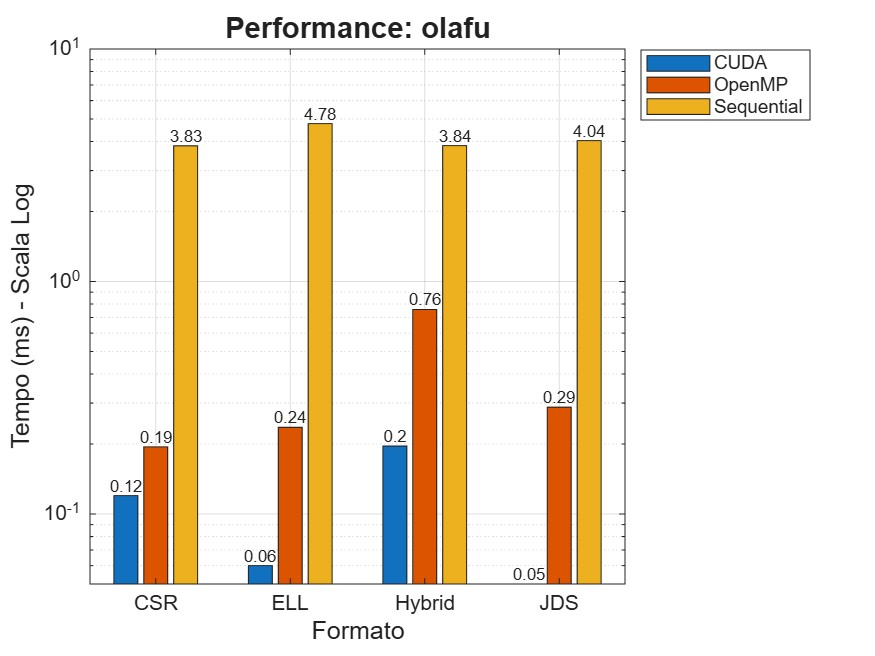
\includegraphics[width=\linewidth]{olafu.jpg} 
        \caption{Matrix: \texttt{olafu}}
        \label{fig:olafu}
    \end{subfigure}
    \hfill
    \begin{subfigure}{0.48\textwidth}
        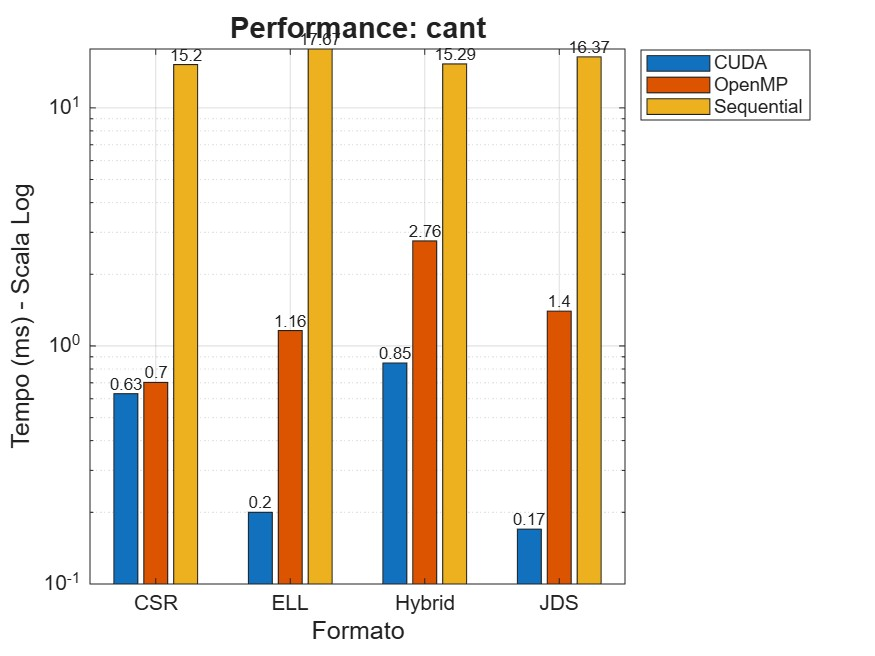
\includegraphics[width=\linewidth]{cant.jpg}
        \caption{Matrix: \texttt{cant}}
        \label{fig:cant}
    \end{subfigure}
    \caption{Performance on structured matrices. ELL and JDS shine on CUDA.}
    \label{fig:structured}
\end{figure}

\subsubsection{Irregular and Sparse Matrices: \texttt{memsplus} and \texttt{scircuit}}
\texttt{memsplus} (Figure \ref{fig:memplus}) is a critical test case. It has a low average degree but high variance. 
\begin{itemize}
    \item The ELL Penalty: Notice the ELL bar on \texttt{scircuit} (Figure \ref{fig:scircuit}) and \texttt{memsplus}. It is orders of magnitude slower compared to CSR. On \texttt{scircuit}, ELL takes 2.73 ms vs 0.07 ms for CSR. This visualizes the memory bandwidth wasted on padding.
    \item Hybrid Efficiency: The Hybrid format (0.02 ms on \texttt{memsplus}) matches the speed of CSR, proving it successfully handles irregularity without the memory penalty of ELL.
\end{itemize}

\begin{figure}[H]
    \centering
    \begin{subfigure}{0.48\textwidth}
        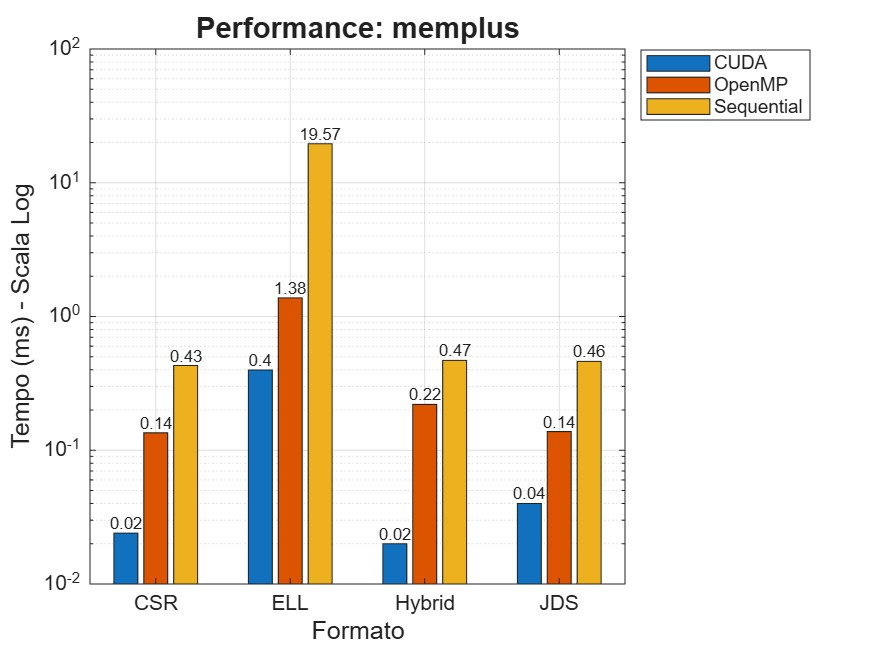
\includegraphics[width=\linewidth]{memplus.jpg} 
        \caption{Matrix: \texttt{memsplus}}
        \label{fig:memplus}
    \end{subfigure}
    \hfill
    \begin{subfigure}{0.48\textwidth}
        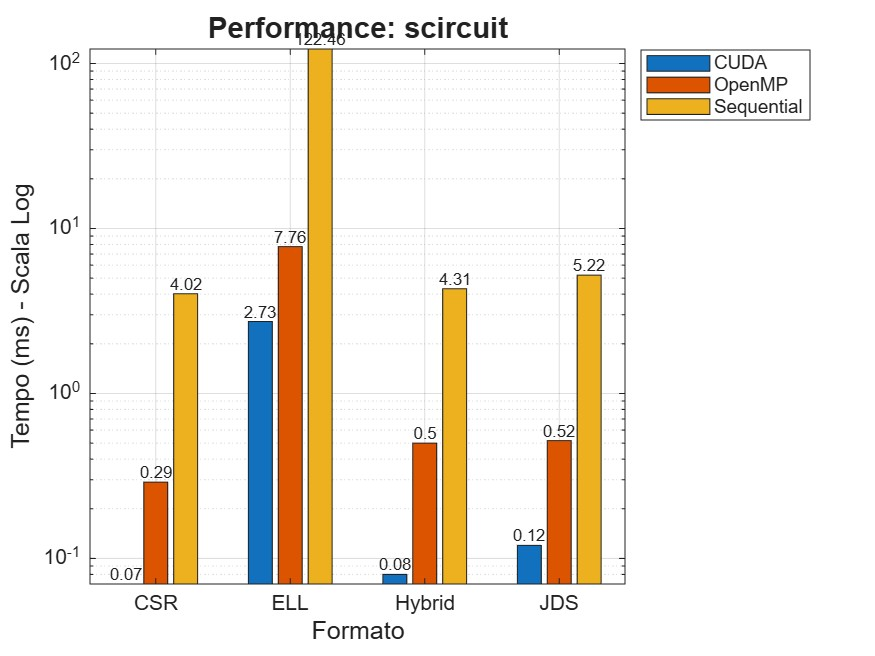
\includegraphics[width=\linewidth]{scircuit.jpg}
        \caption{Matrix: \texttt{scircuit}}
        \label{fig:scircuit}
    \end{subfigure}
    \caption{Performance on irregular matrices. Note the massive penalty of ELL due to padding.}
\end{figure}

\subsubsection{Power-Law Graphs: \texttt{web-Google}}
The \texttt{web-Google} matrix (Figure \ref{fig:web-Google}) represents the ultimate stress test. 

\begin{itemize}
    \item ELL Failure: The graph shows no bar for ELL. The format failed due to excessive memory requirements ($>2$GB for a 60MB matrix), confirming our theoretical analysis.
    \item Hybrid Victory: Surprisingly, the Hybrid format achieves the best performance on CUDA (0.93 ms), beating CSR (1.04 ms). This demonstrates that moving the few "hub" nodes (dense rows) into the COO structure allows the GPU to process the rest of the web graph very efficiently.
\end{itemize}

\begin{figure}[H]
    \centering
    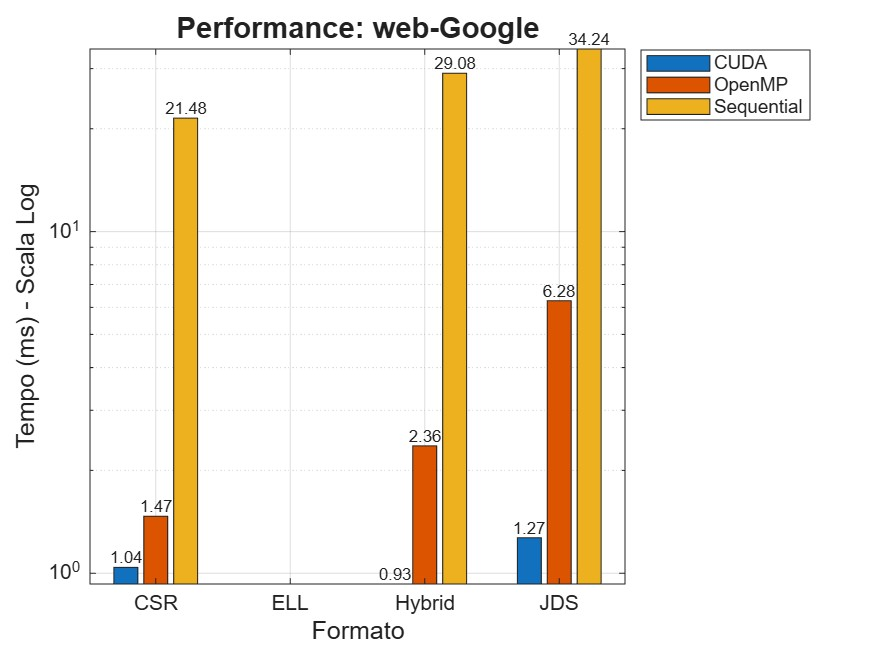
\includegraphics[width=0.7\textwidth]{web-Google.jpg}
    \caption{Performance on \texttt{web-Google}. ELL is missing (OOM). Hybrid outperforms CSR.}
    \label{fig:web-Google}
\end{figure}
\section{Conclusion}
The project demonstrated that handling irregularity is the main challenge in SpMV on GPUs.
\begin{itemize}
    \item ELL is ideal for structured grid problems but unstable for real-world graphs.
    \item Hybrid is a robust compromise that fits in memory but incurs atomic overhead.
    \item JDS proves to be the superior format for highly irregular (Power-Law) matrices on GPU, solving both memory coalescing and load balancing issues, at the cost of a pre-processing step (sorting rows).
\end{itemize}

While OpenMP provides a simple parallelization for CPUs, the massive bandwidth of the GPU (HBM/GDDR) allows for significant speedups, provided the correct storage format is chosen to match the data structure.

\appendix
\section{Appendix: Hardware Specifications}
The experiments were conducted on the following system:

\begin{table}[H]
    \centering
    \begin{tabular}{|l|l|}
    \hline
    \textbf{Component} & \textbf{Specification} \\
    \hline
    CPU & AMD Ryzen 5 3600 6-Core Processor  \\
    \hline
    RAM & 16,0 GB \\
    \hline
    GPU & NVIDEA GeForce RTX 3050 \\
    \hline
    CUDA Cores & 2560 \\
    \hline
    OS & Windows 11 \\
    \hline
    \end{tabular}
    \caption{System Specifications}
\end{table}

\end{document}